\documentclass[tikz,border=5pt]{standalone}
\usepackage{luatexja}
\usepackage[hiragino-pron]{luatexja-preset}
\usepackage{amsmath,amssymb,bm}
\usetikzlibrary{arrows.meta,decorations.markings}

\begin{document}
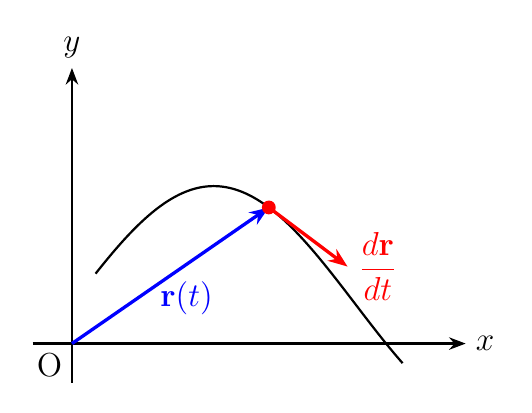
\begin{tikzpicture}[every node/.style={font=\large}]
  % Axes
  \draw[-{Stealth[length=6pt]}, thick] (-0.5,0) -- (5,0) node[right] {$x$};
  \draw[-{Stealth[length=6pt]}, thick] (0,-0.5) -- (0,3.5) node[above] {$y$};
  \node[below left] at (0,0) {O};

  % Parametric curve (black)
  \draw[thick, domain=0.3:4.2, samples=100]
    plot (\x, {0.5 + 1.5*sin(\x*50)});

  % Position vector from origin to point (blue)
  \draw[-{Stealth[length=7pt]}, very thick, blue] (0,0) -- (2.5, {0.5 + 1.5*sin(2.5*50)});
  \node[blue, below right] at (1.0, {0.3 + 0.75*sin(2.5*50)}) {$\mathbf{r}(t)$};

  % Point on curve
  \fill[red] (2.5, {0.5 + 1.5*sin(2.5*50)}) circle (2.5pt);

  % Tangent vector
  \draw[-{Stealth[length=7pt]}, very thick, red] (2.5, {0.5 + 1.5*sin(2.5*50)})
    -- ++(1.0, {1.5*50*cos(2.5*50)*0.01745*1.0})
    node[right] {$\dfrac{d\mathbf{r}}{dt}$};
\end{tikzpicture}
\end{document}
